\section{Buck-converter\label{Buck-C}}

The task of a buck converter is to decrease the input voltage. The needed components are a DC-source for the input voltage, two switches (a diode and a transistor), an inductor, a capacitor and a load. The equivalent diagram in figure \ref{Buck-converter} illustrates a buck-converter. 

\begin{figure}[htbp]
	\begin{center}
		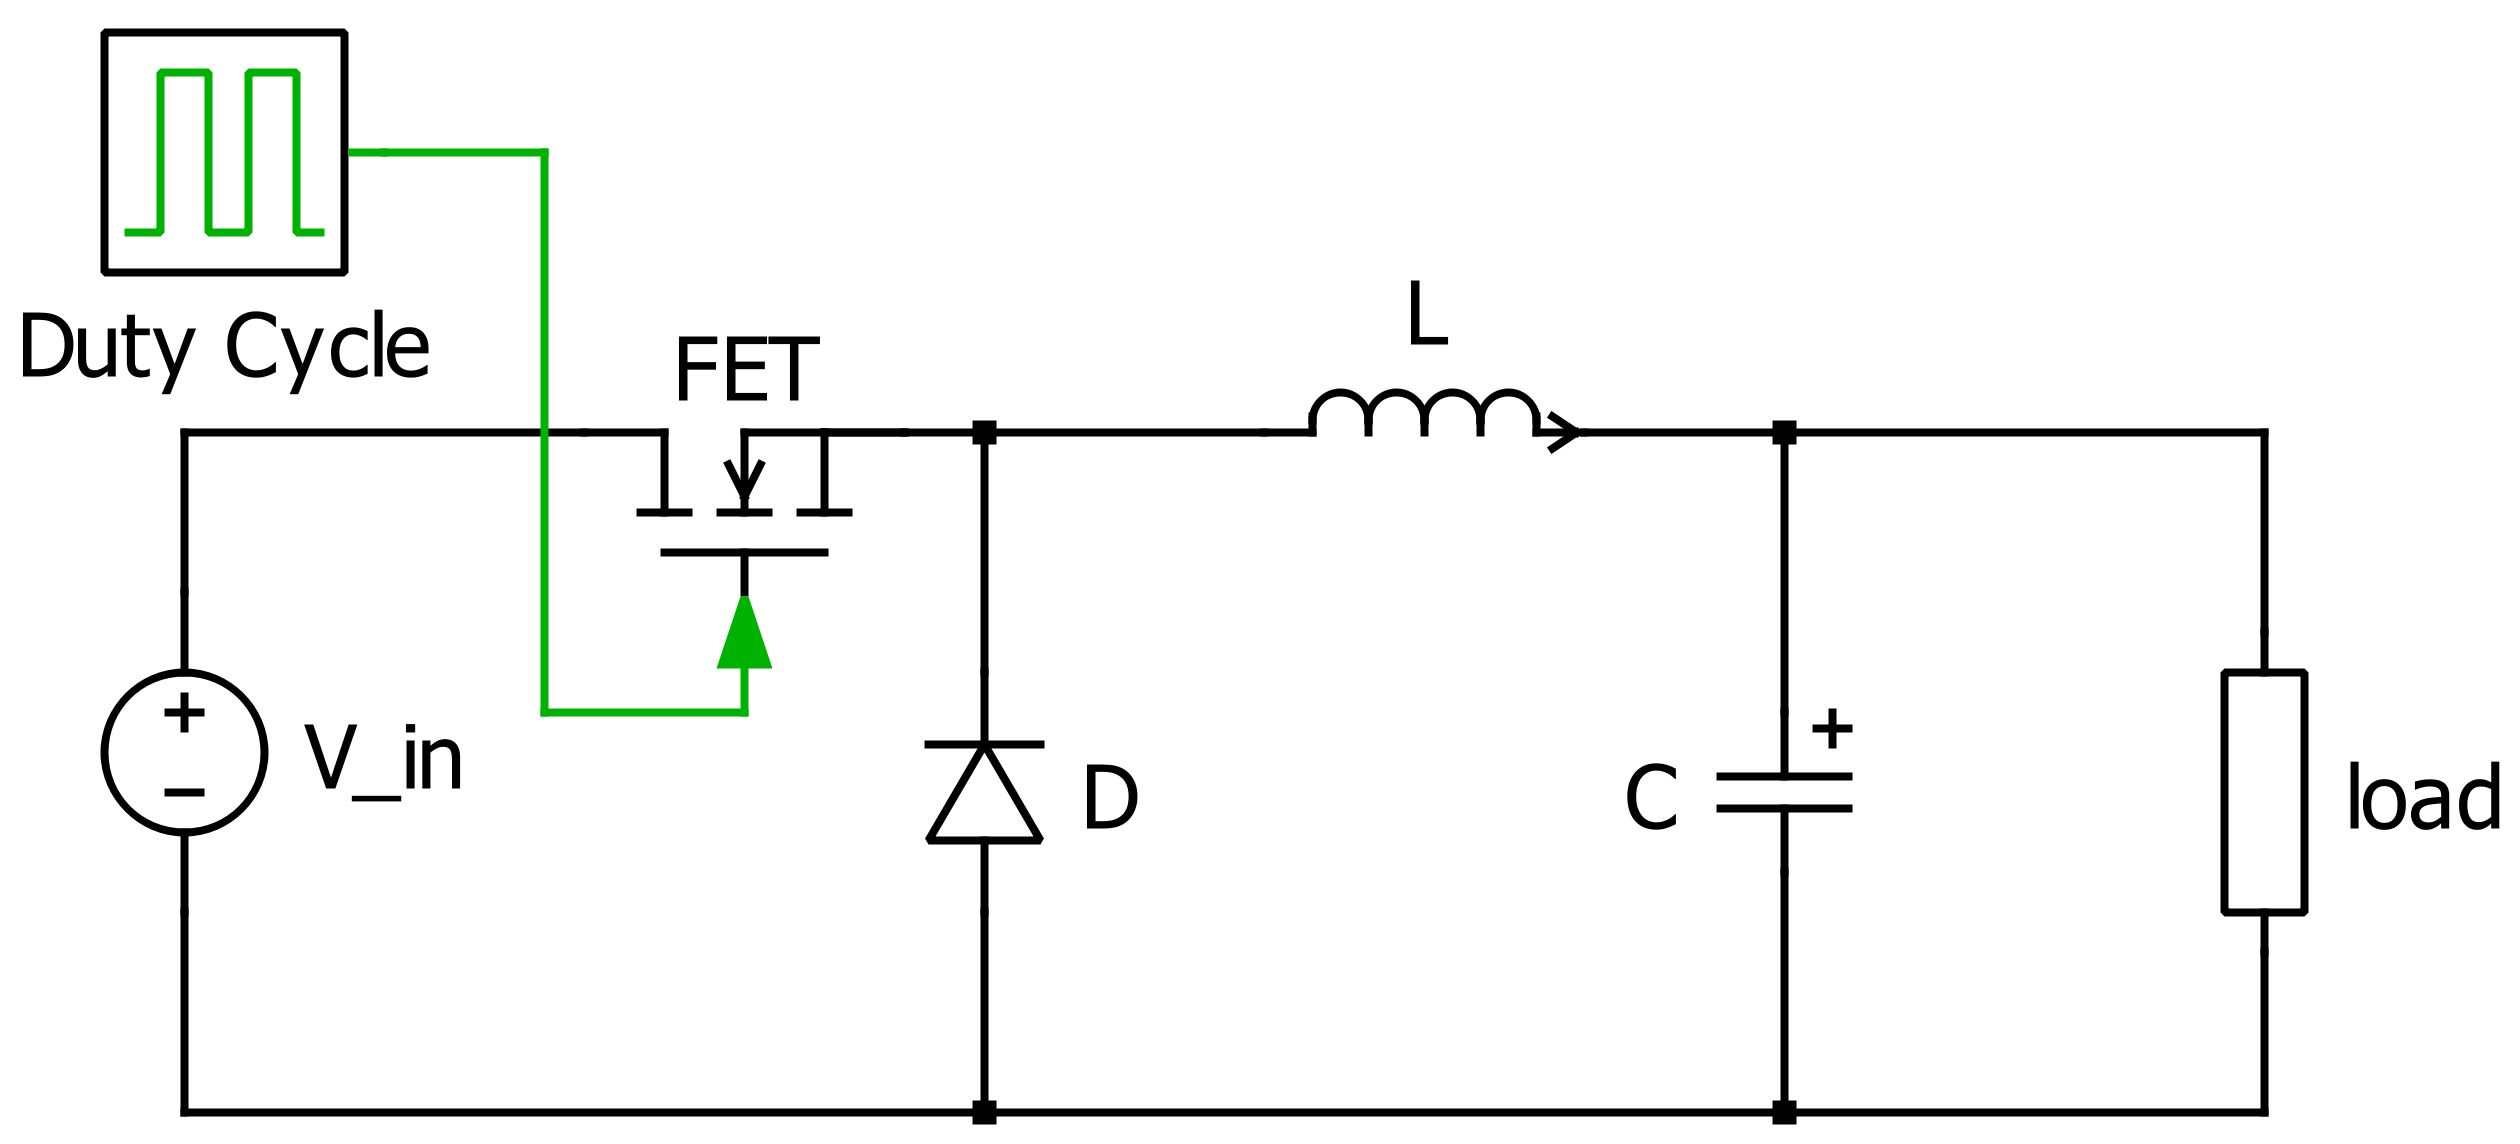
\includegraphics[width=0.7\textwidth]{../Pictures/Buck-converter}
		\caption{Buck-converter.}
		\label{Buck-converter}
	\end{center}	
\end{figure}

A buck-converter performs in two operating states. 
%In both states have been an approach that the converter is in steady state. Because of that the average of a value is constant and we can assume a DC-voltage at the load. %
During the first state, the MOSFET is conducting and the diode is working as an open-circuit, the voltage drop will then appear on the inductor and on the load. Since the voltage is split, there is a lower voltage on the load. In addition the capacitor and the inductor are charging energy. In the second state the MOSFET is switched off and the current flow trough the diode. The inductor will work as a current source and %(feeds the closed circuit with current. )
the capacitor will supply the load with energy\cite{schematicbuckandboost}.
%At the case, that the MOSFET conducts current, the diode will be closed and the voltage drops at the inductor. Thus,  you can measure a lower voltage at the load. Besides that, the capacitor is loaded energy and the inductor is loaded current. If the MOSFET doesn't conduct current, the inductor will work as a current source and feeds the closed circuit with current. The capacitor is discharging and supplied the load.

The advantage for using the buck converter is that the structure is very simple and you need one power switch. The size for the component is small and the cost for this is low. Furthermore, the buck converter has a high efficiency of over 90 \%\cite{datasheetbuck}. A disadvantage  is the output voltage ripple is high. With an electronic filter it is possible to reduce the ripple\cite{advantagebuck}.
%%http://www.completepowerelectronics.com/buck-converter-tutorial-topology-working-advantages-applications/

\section{Boost-converter\label{Boost-C}}

A boost converter produces a higher output voltage in comparison to the input voltage. The circuit consists of two switches, which obtains a diode and a tr, an inductor, a capacitor, a load and a DC-Source for the input voltage. Figure \ref{Boost-converter} shows an equivalent circuit diagram with the aforementioned components. %%\cite{Reddy2011}

\begin{figure}[htbp]
	\begin{center}
		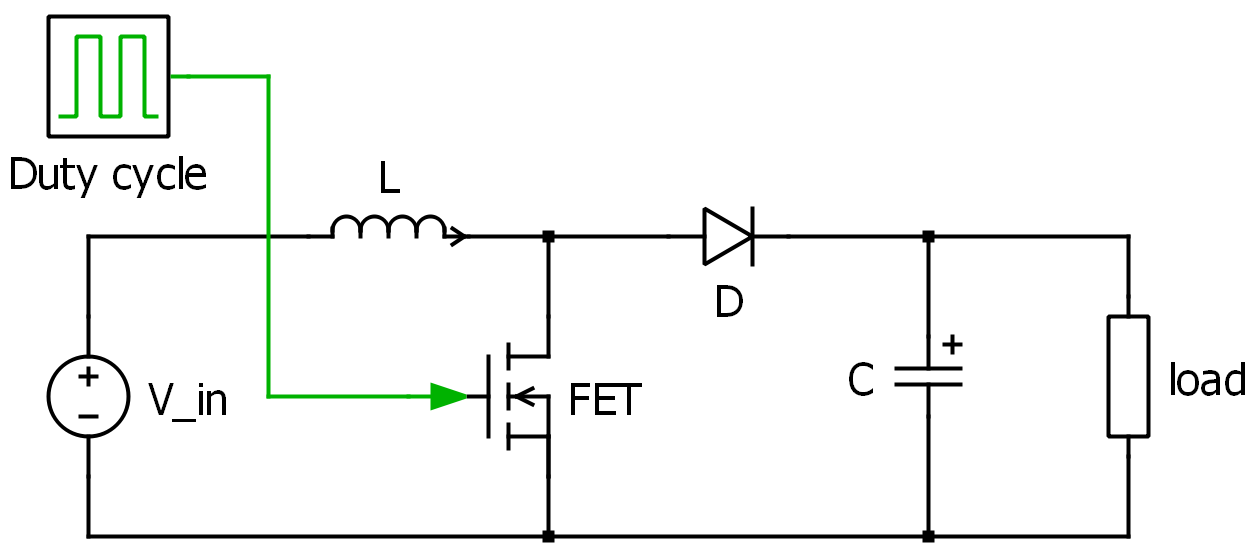
\includegraphics[width=0.7\textwidth]{../Pictures/Boost-converter}
		\caption{Boost-converter.}
		\label{Boost-converter}
	\end{center}	
\end{figure}

If the MOSFET is on , the current flows only trough the inductors because the diode  is working as an open-circuit.Energy will be stored in the inductor magnetic field. Meanwhile, the capacitor releases the stored energy to the load.% Thus, the output voltage decreases slowly.%
In the other case, when the MOSFET doesn’t conduct, the current flows trough the inductor, diode, capacitor and the load. The polarity of the inductor will reverse because of the instant change of the current flow.%higher impedance in this state.
Therefore, the inductor voltage can be added to the input voltage and the output voltage will be higher than the input voltage. Furthermore, the capacitor is recharging\cite{schematicbuckandboost}.

An advantage for a boost converter is that it can raise the output voltage without help from a transformer. The size for the inductor and capacitor will have to be large, if you want an output without voltage ripple.\cite{advantageboost}. %Furthermore changing the output voltage to big difference potential in the duty cycle can destroy components\cite{advantageboost}.
 
